% Editable vector reconstruction of the supplied figure.
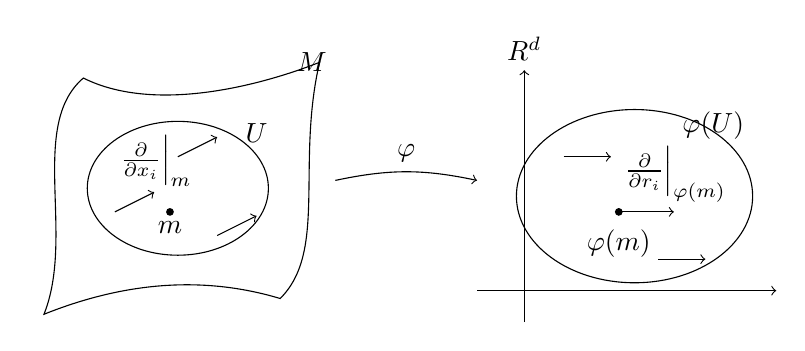
\begin{tikzpicture}

\draw (-.5,-.5)..controls(-.1,.5)and(-.7,1.9)..(0,2.5)..controls(1,2)and(2.5,2.5)..(3,2.7)..controls(2.7,1.4)and(3.1,.3)..(2.5,-.3)..controls(1.5,0)and(.5,-.1)..cycle;
\node at(2.9,2.7){$M$};\draw (1.2,1.1) ellipse(1.15 and .85);\node at(2.2,1.8){$U$};
\foreach \a/\b in {.4/.8,1.2/1.5,1.7/.5}{\draw[->](\a,\b)--++(.5,.25);}
\fill(1.1,.8)circle(1.4pt)node[below]{$m$};\node[above left] at(1.5,1){$\left.\frac\partial{\partial x_i}\right|_m$};
\draw[->](3.2,1.2)to[bend left=12]node[above]{$\varphi$}(5,1.2);
\draw[->](5,-.2)--(8.8,-.2);\draw[->](5.6,-.6)--(5.6,2.6)node[above]{$\mathbb R^d$};
\draw(7,1)ellipse(1.5 and 1.1);\node at(8,1.9){$\varphi(U)$};
\foreach \a/\b in {6.1/1.5,7.3/.2}{\draw[->](\a,\b)--++(.6,0);}
\fill(6.8,.8)circle(1.4pt)node[below=3pt]{$\varphi(m)$};\draw[->](6.8,.8)--(7.5,.8)node[above]{$\left.\frac\partial{\partial r_i}\right|_{\varphi(m)}$};
\end{tikzpicture}
